\section{Preisstabilit�t}
\subsection{Inflation und Deflation \ho{Ho9}}
  F�r eine Inflation braucht es eine Lohn-Preis-Spirale und eine Nationalbank
  die das ganze unterst�tzt. \ho{Ho9 F15}
  \begin{multicols}{2}
	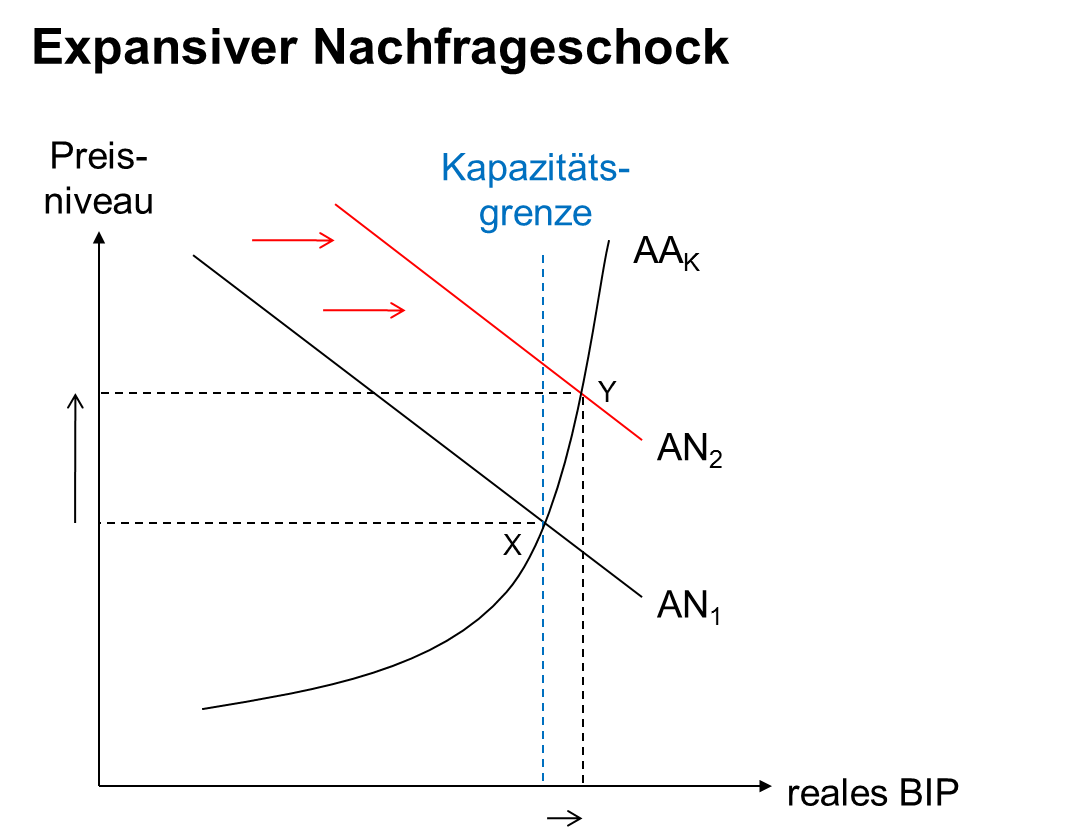
\includegraphics[width=9cm]{./bilder/h09f08.png} \\
	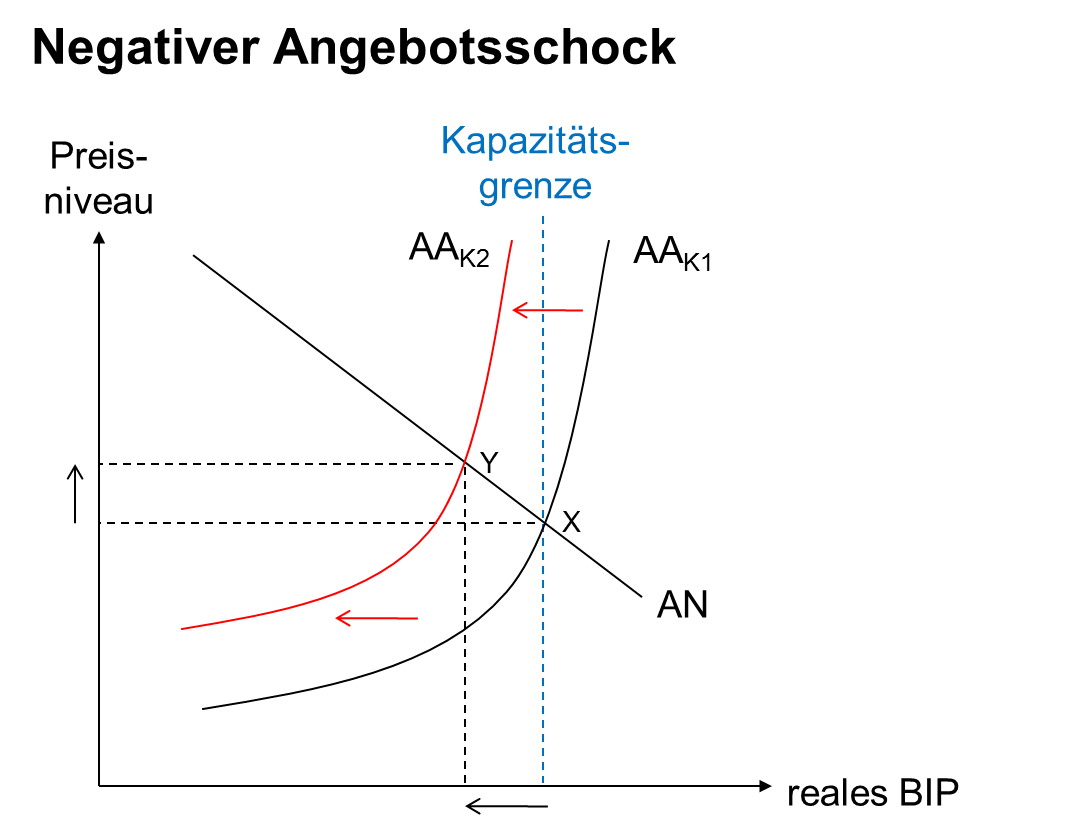
\includegraphics[width=9cm]{./bilder/h09f11.png}
\end{multicols}
\subsection{Geld \ho{Ho10}}
\subsubsection{Geldmengenkonzepte der Schweiz \ho{Ho10 F8}}
  Notenbank legt nur $m_0$ fest. Der rest ist durch Kreditanleihen der
  Privatbanken.
  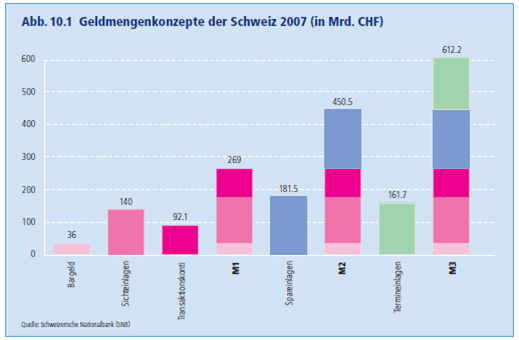
\includegraphics[width=18cm]{./bilder/h10f08.png}
